\documentclass[a4paper,11pt]{article}

\usepackage[utf8]{inputenc}
\usepackage[italian]{babel}
\usepackage[sfdefault]{roboto}
\usepackage{layaureo} % reduce margins
\usepackage{url}
\usepackage{hyperref}
\usepackage{graphicx}
\usepackage{float}
\usepackage{alertmessage}

% Setup
\hypersetup{hidelinks}


% Document
\begin{document}
\title{IR Extender}
\author{Davide Pizzoli \\ Stefano Zenaro}
\date{Aprile 2022}

\pagenumbering{gobble}

% Title
\begin{titlepage}
  \maketitle
  \thispagestyle{empty}
\end{titlepage}

% Table of contents
\tableofcontents
\addcontentsline{toc}{section}{Indice}
\clearpage

\pagenumbering{arabic}

% Contents
\section{Introduzione}

  Il seguente documento descrive come realizzare un IR Extender.

  \subsection{Funzionamento}

    \begin{figure}[H]
      \centering
      \includegraphics[width=\textwidth,height=\textheight,keepaspectratio]{assets/ir_extender}
      \caption{IR Extender}
    \end{figure}

    % TODO: describe how to use the IR Extender

  \subsection{Componenti}

    \begin{itemize}
      \item IR Receiver
      \item IR Transmitter
      \item ESP32 / ESP8266 * 2
      \item Jumpers * 6
      \item Breadboard * 2
    \end{itemize}

  \subsection{Online Services}

    \begin{itemize}
      \item Broker MQTT (es. \href{https://www.hivemq.com/}{HiveMQ})
    \end{itemize}

  \alertinfo{Il Ricevitore e Trasmettitore possono essere collegati a due reti WiFi differenti.}


\section{Ricevitore}
\label{sec:receiver}

  Il dispositivo ricevitore si occupa di:

  \begin{enumerate}
    \item Ricevere un segnale infrarossi da un telecomando
    \item Inviare l'informazione del segnale infrarossi, utilizzando la rete Wi-Fi, con il protocollo MQTT al Broker MQTT
  \end{enumerate}

  \subsection{Circuito}

    \begin{figure}[H]
      \centering
      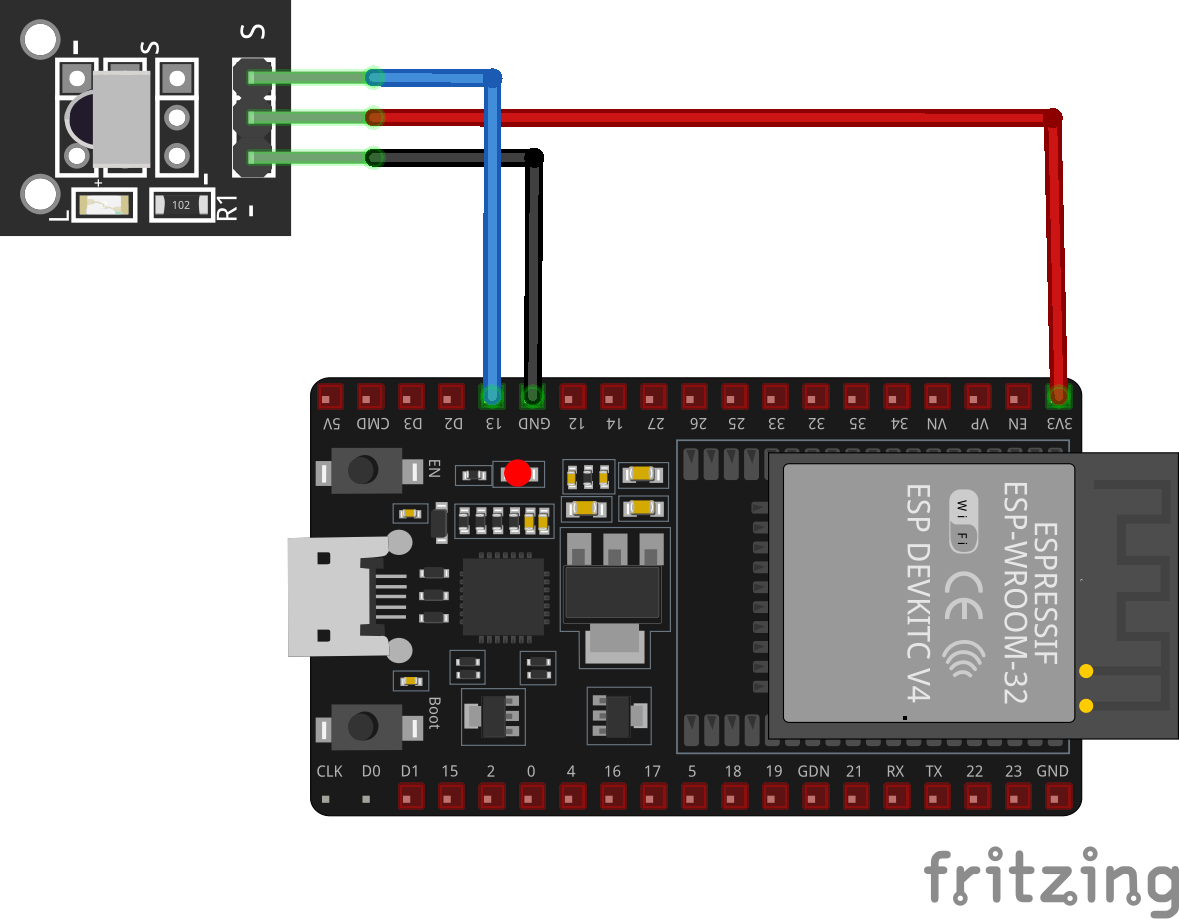
\includegraphics[width=0.5\textwidth,height=\textheight,keepaspectratio]{assets/receiver_fritzing}
      \caption{Circuito Ricevitore}
    \end{figure}

  \subsection{Configurazione}

  \begin{enumerate}
    \item Aprire la cartella \texttt{receiver/src}
    \item Rinominare il file \texttt{secrets.h.sample} in \texttt{secrets.h} e aprirlo
    \item Inserire i dati di accesso della rete WiFi e del \hyperref[sec:Broker]{Broker MQTT}
  \end{enumerate}


\section{Trasmettitore}
\label{sec:transmitter}

  Il dispositivo trasmettitore si occupa di:

  \begin{enumerate}
    \item Ricevere l'informazione dal Broker MQTT
    \item Inviare il segnale ricevuto tramite il trasmettitore infrarossi
  \end{enumerate}


  \subsection{Circuito}

    \begin{figure}[H]
      \centering
      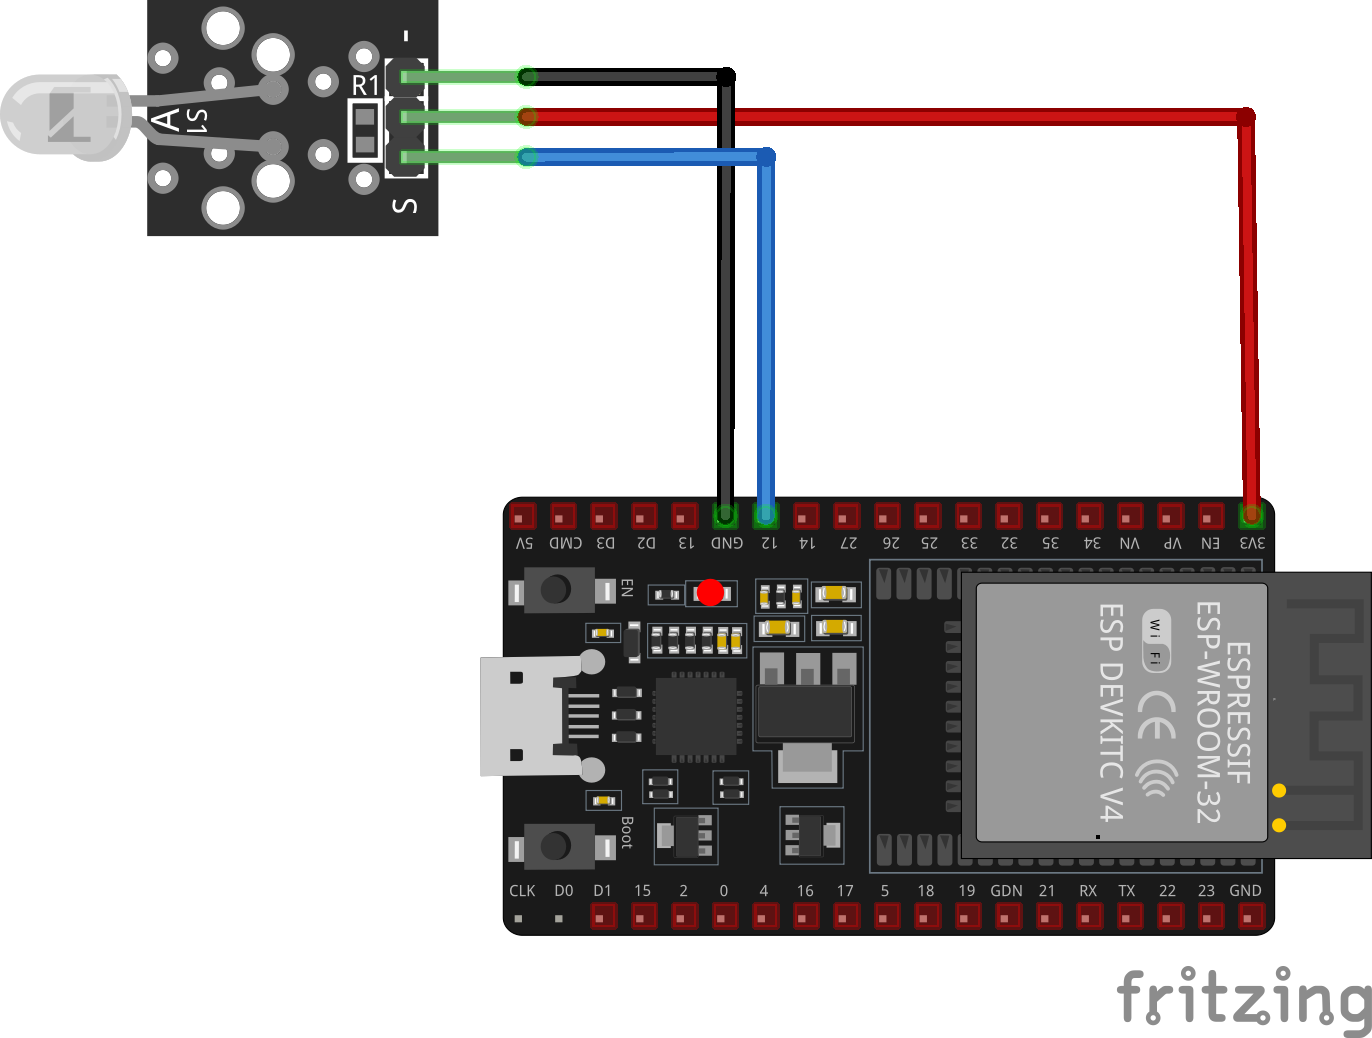
\includegraphics[width=0.5\textwidth,height=\textheight,keepaspectratio]{assets/transmitter_fritzing}
      \caption{Circuito Trasmettitore}
    \end{figure}


  \subsection{Configurazione}

    \begin{enumerate}
      \item Aprire la cartella \texttt{transmitter/src}
      \item Rinominare il file \texttt{secrets.h.sample} in \texttt{secrets.h} e aprirlo
      \item Inserire i dati di accesso della rete WiFi e del \hyperref[sec:Broker]{Broker MQTT}
    \end{enumerate}


\section{Broker MQTT (HiveMQ)}
\label{sec:Broker}

  \subsection{Configurazione}

    \begin{enumerate}
      \item \href{https://console.hivemq.cloud/}{Registrarsi su HiveMQ}
      \item Creare un nuovo \emph{Cluster}
        \begin{figure}[H]
          \centering
          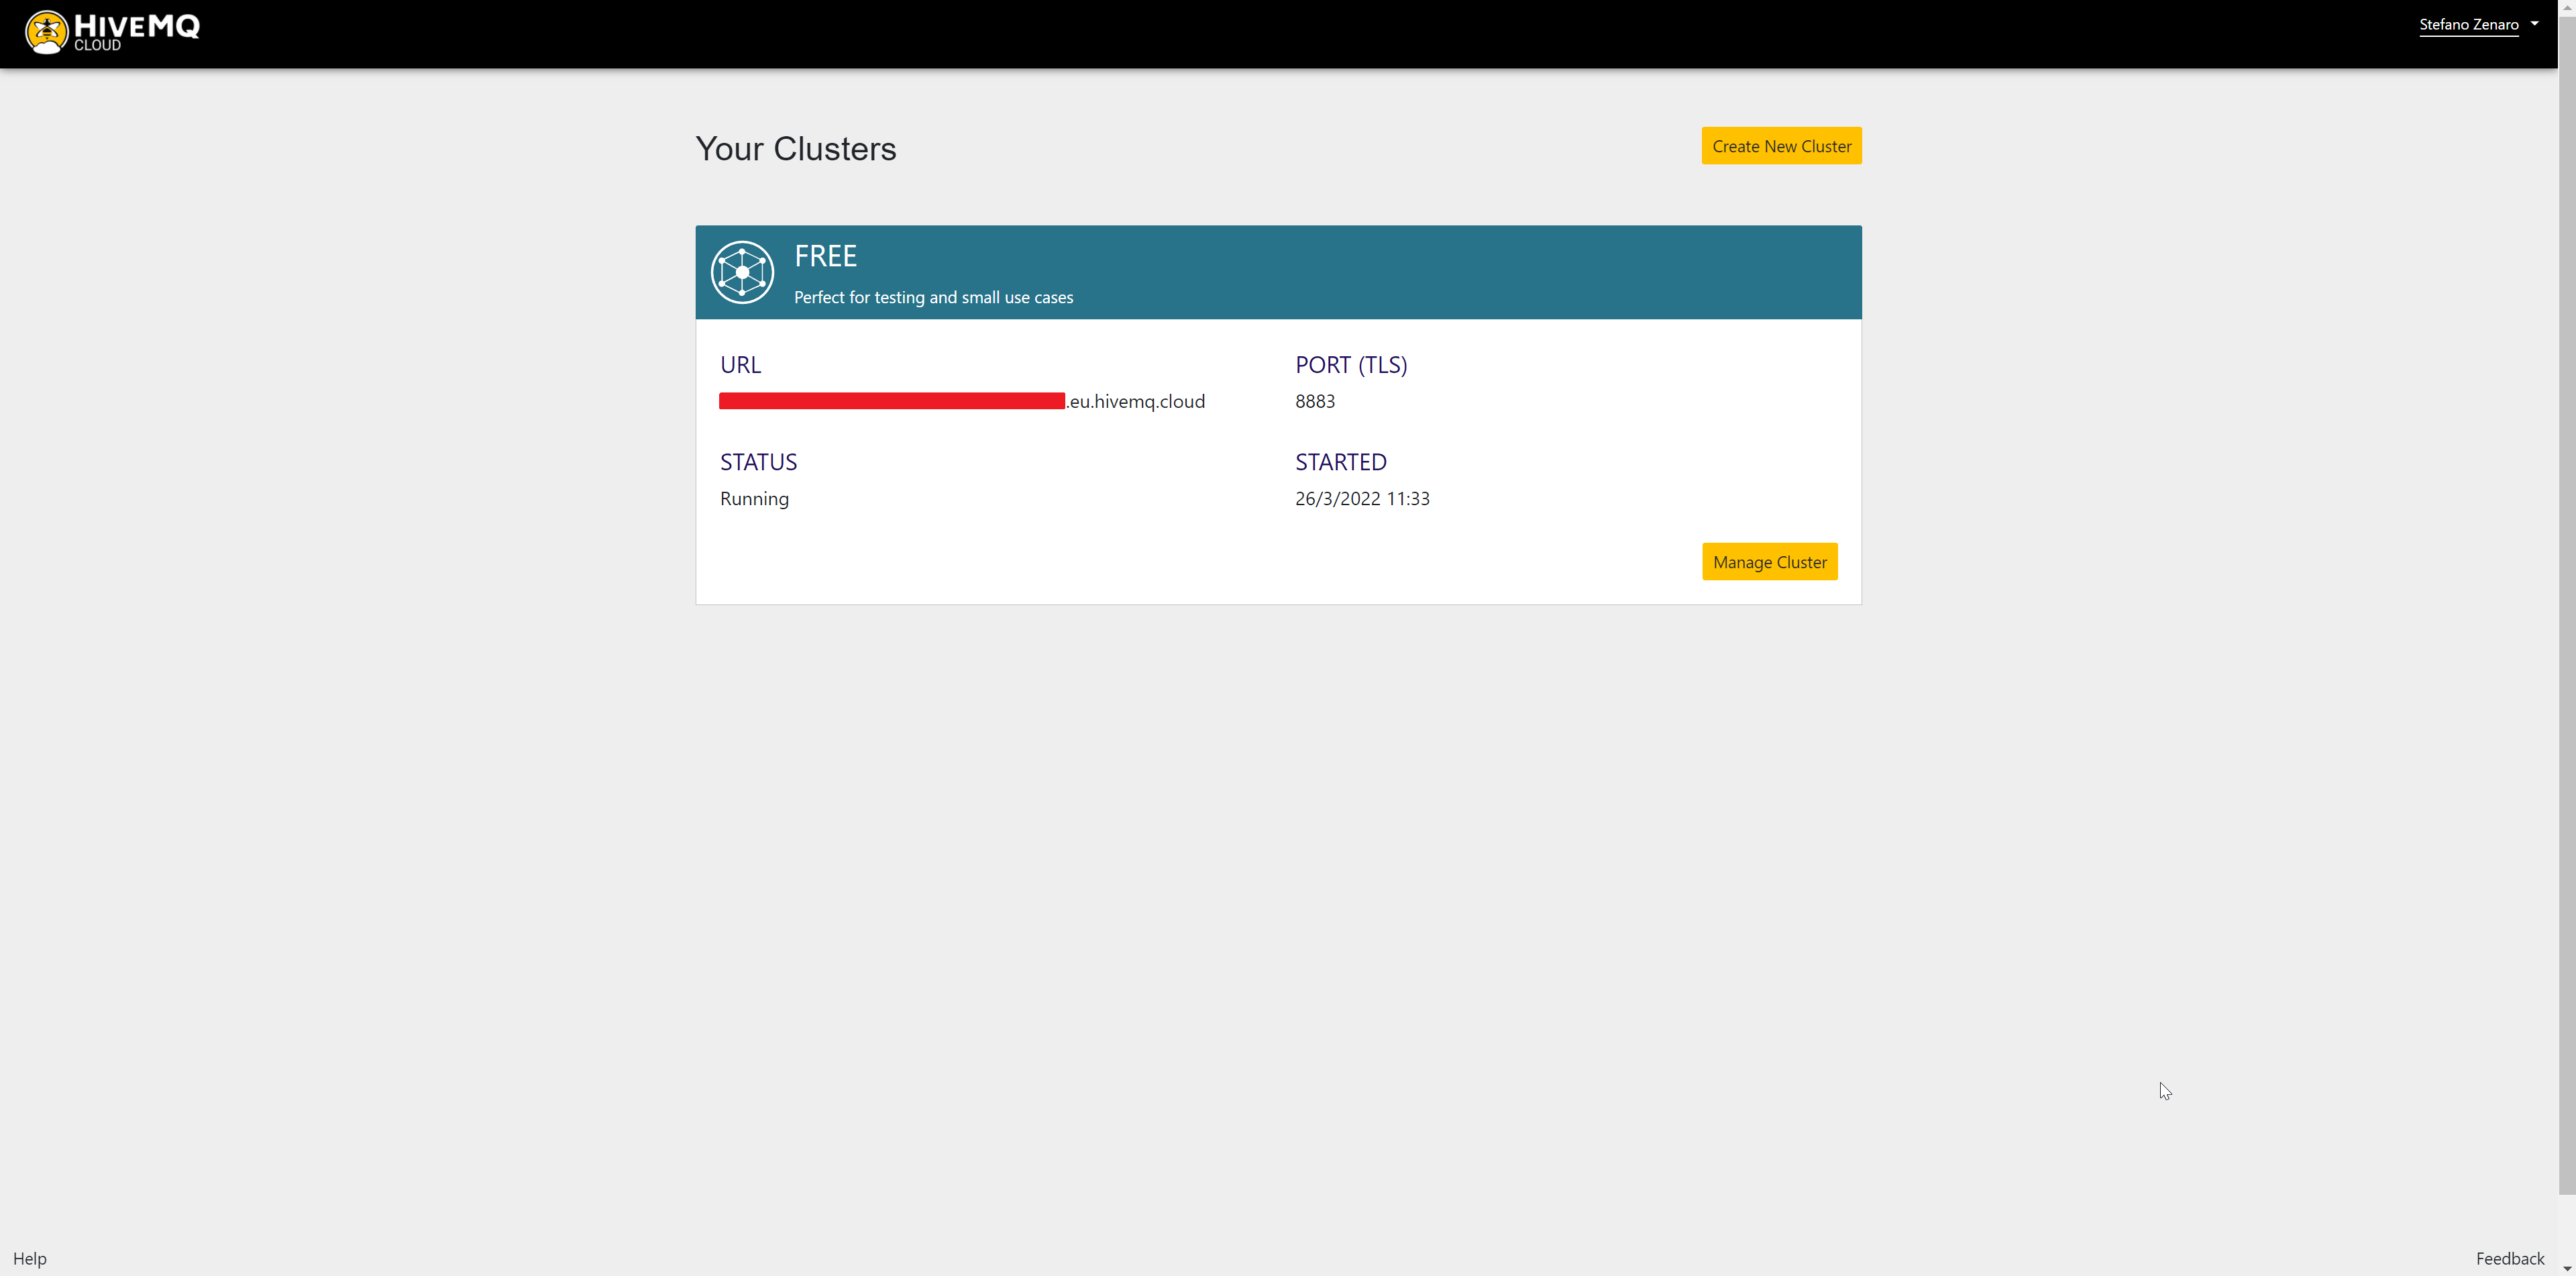
\includegraphics[width=0.8\textwidth,height=\textheight,keepaspectratio]{assets/hivemq_clusters}
        \end{figure}

        Salvarsi l'\emph{URL} del Cluster, che sarà utilizzato per configurare il Ricevitore e il Trasmettitore.

      \item Cliccare su \emph{Manage cluster}
        \begin{figure}[H]
          \centering
          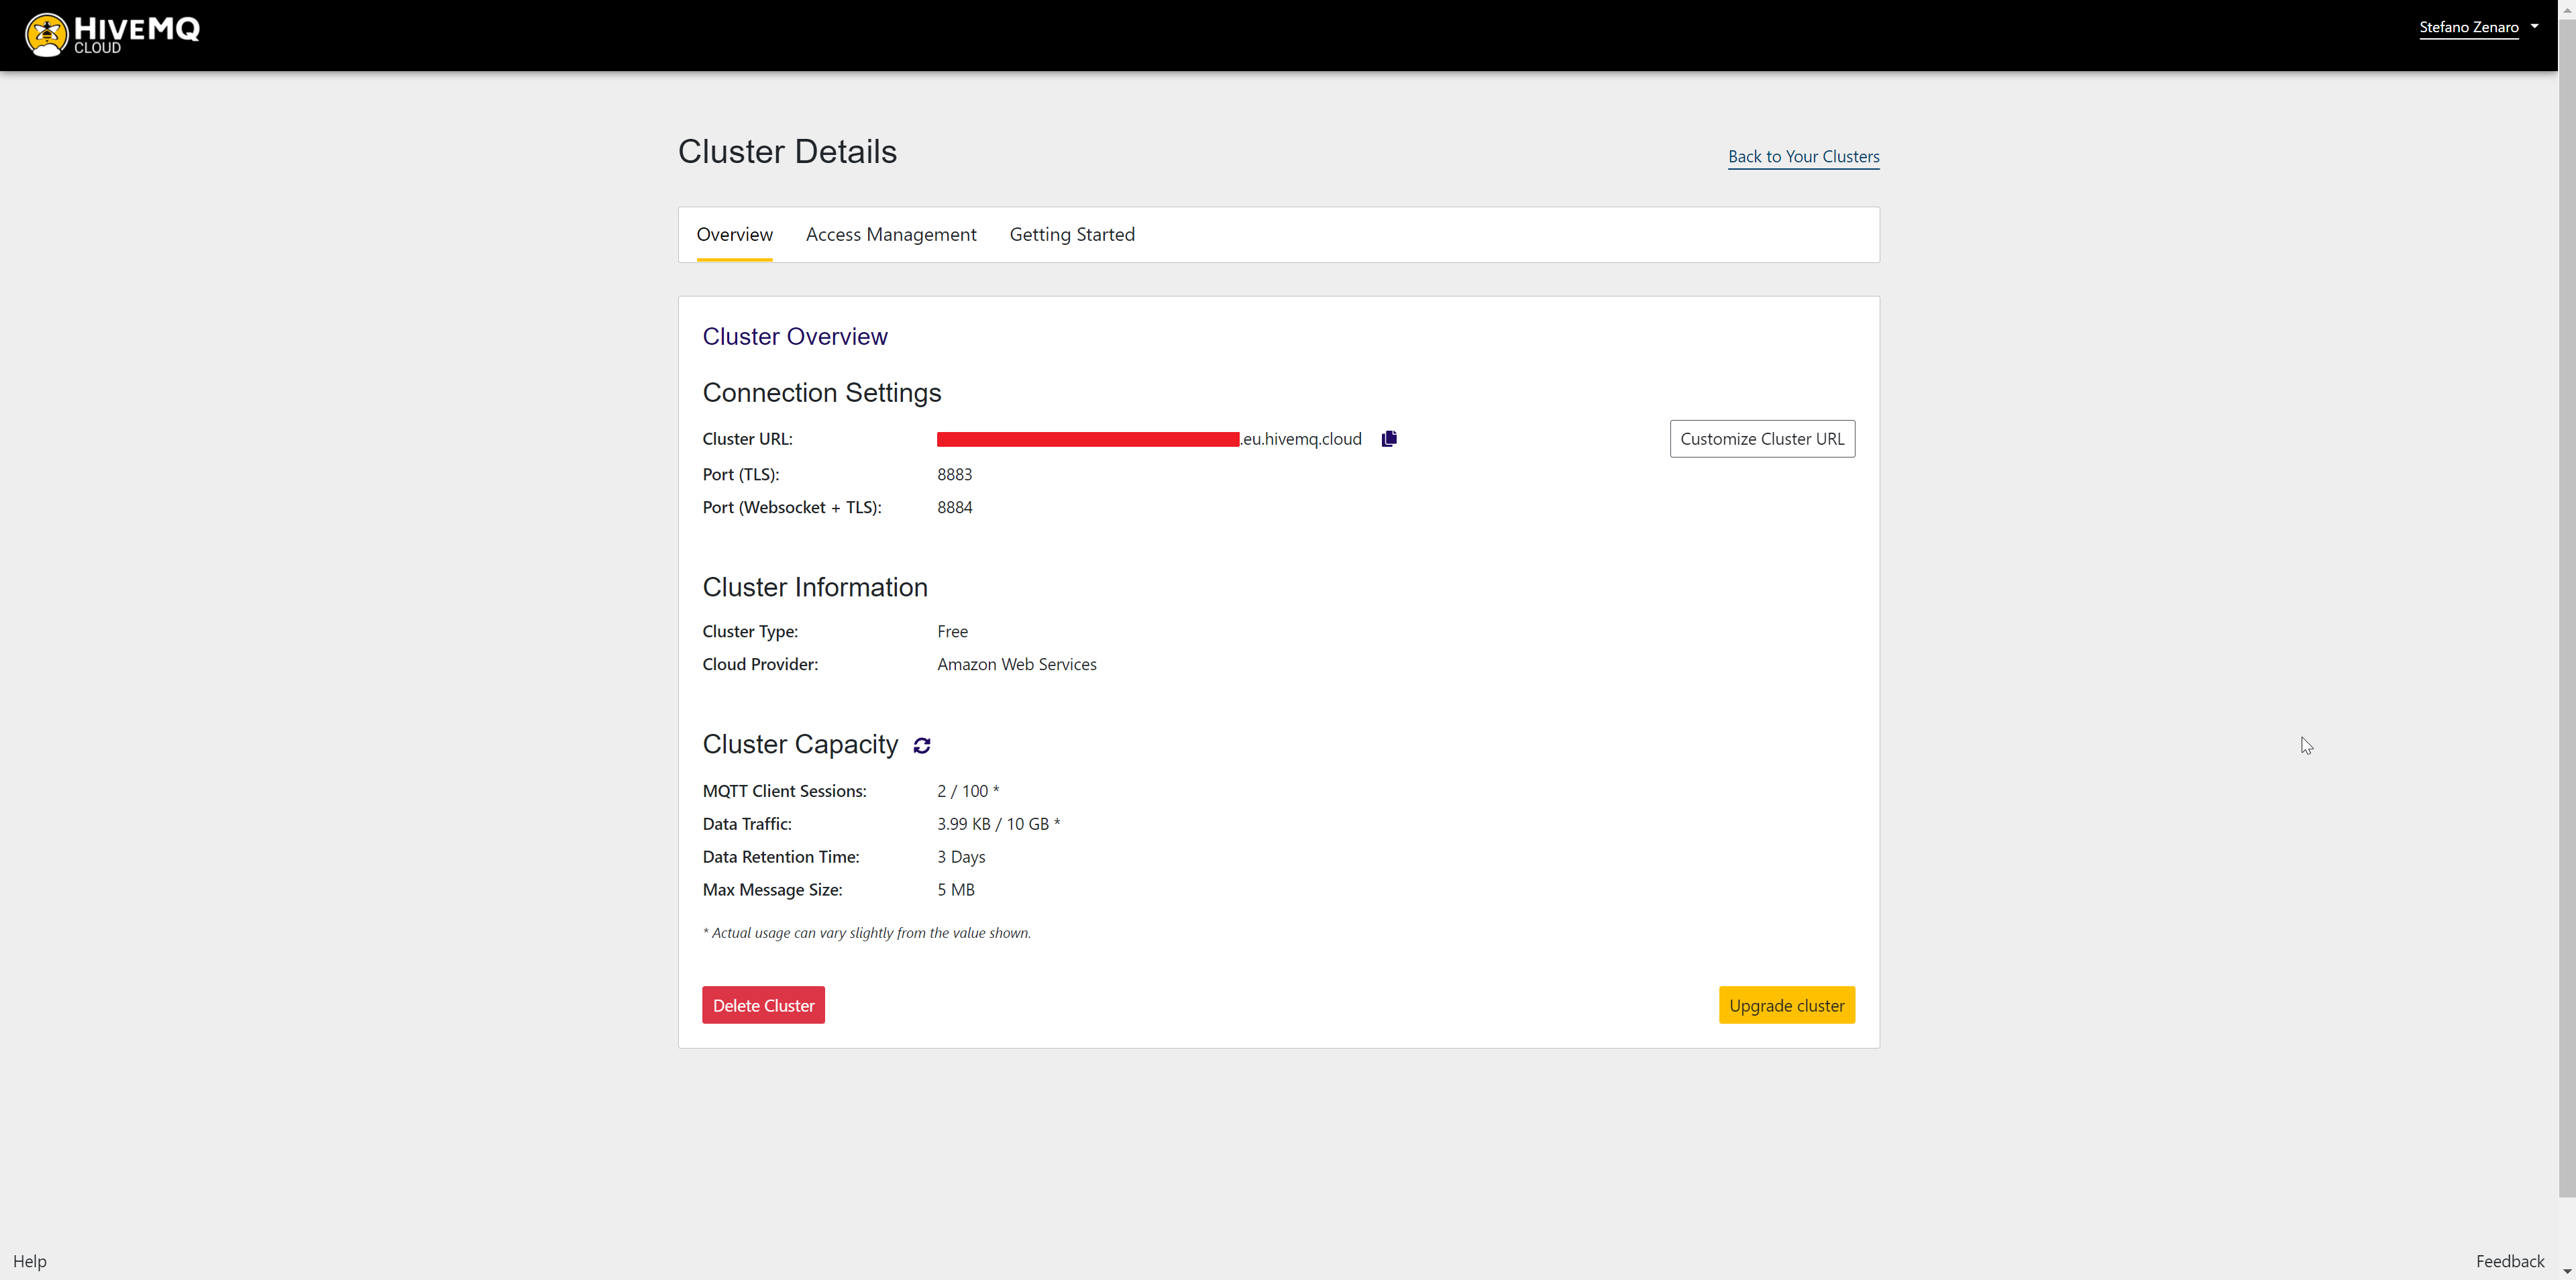
\includegraphics[width=0.8\textwidth,height=\textheight,keepaspectratio]{assets/hivemq_clusterdetails}
        \end{figure}

      \item Nella sezione \emph{Access Management} aggiungere delle credenziali di accesso al \emph{Cluster}
        \begin{figure}[H]
          \centering
          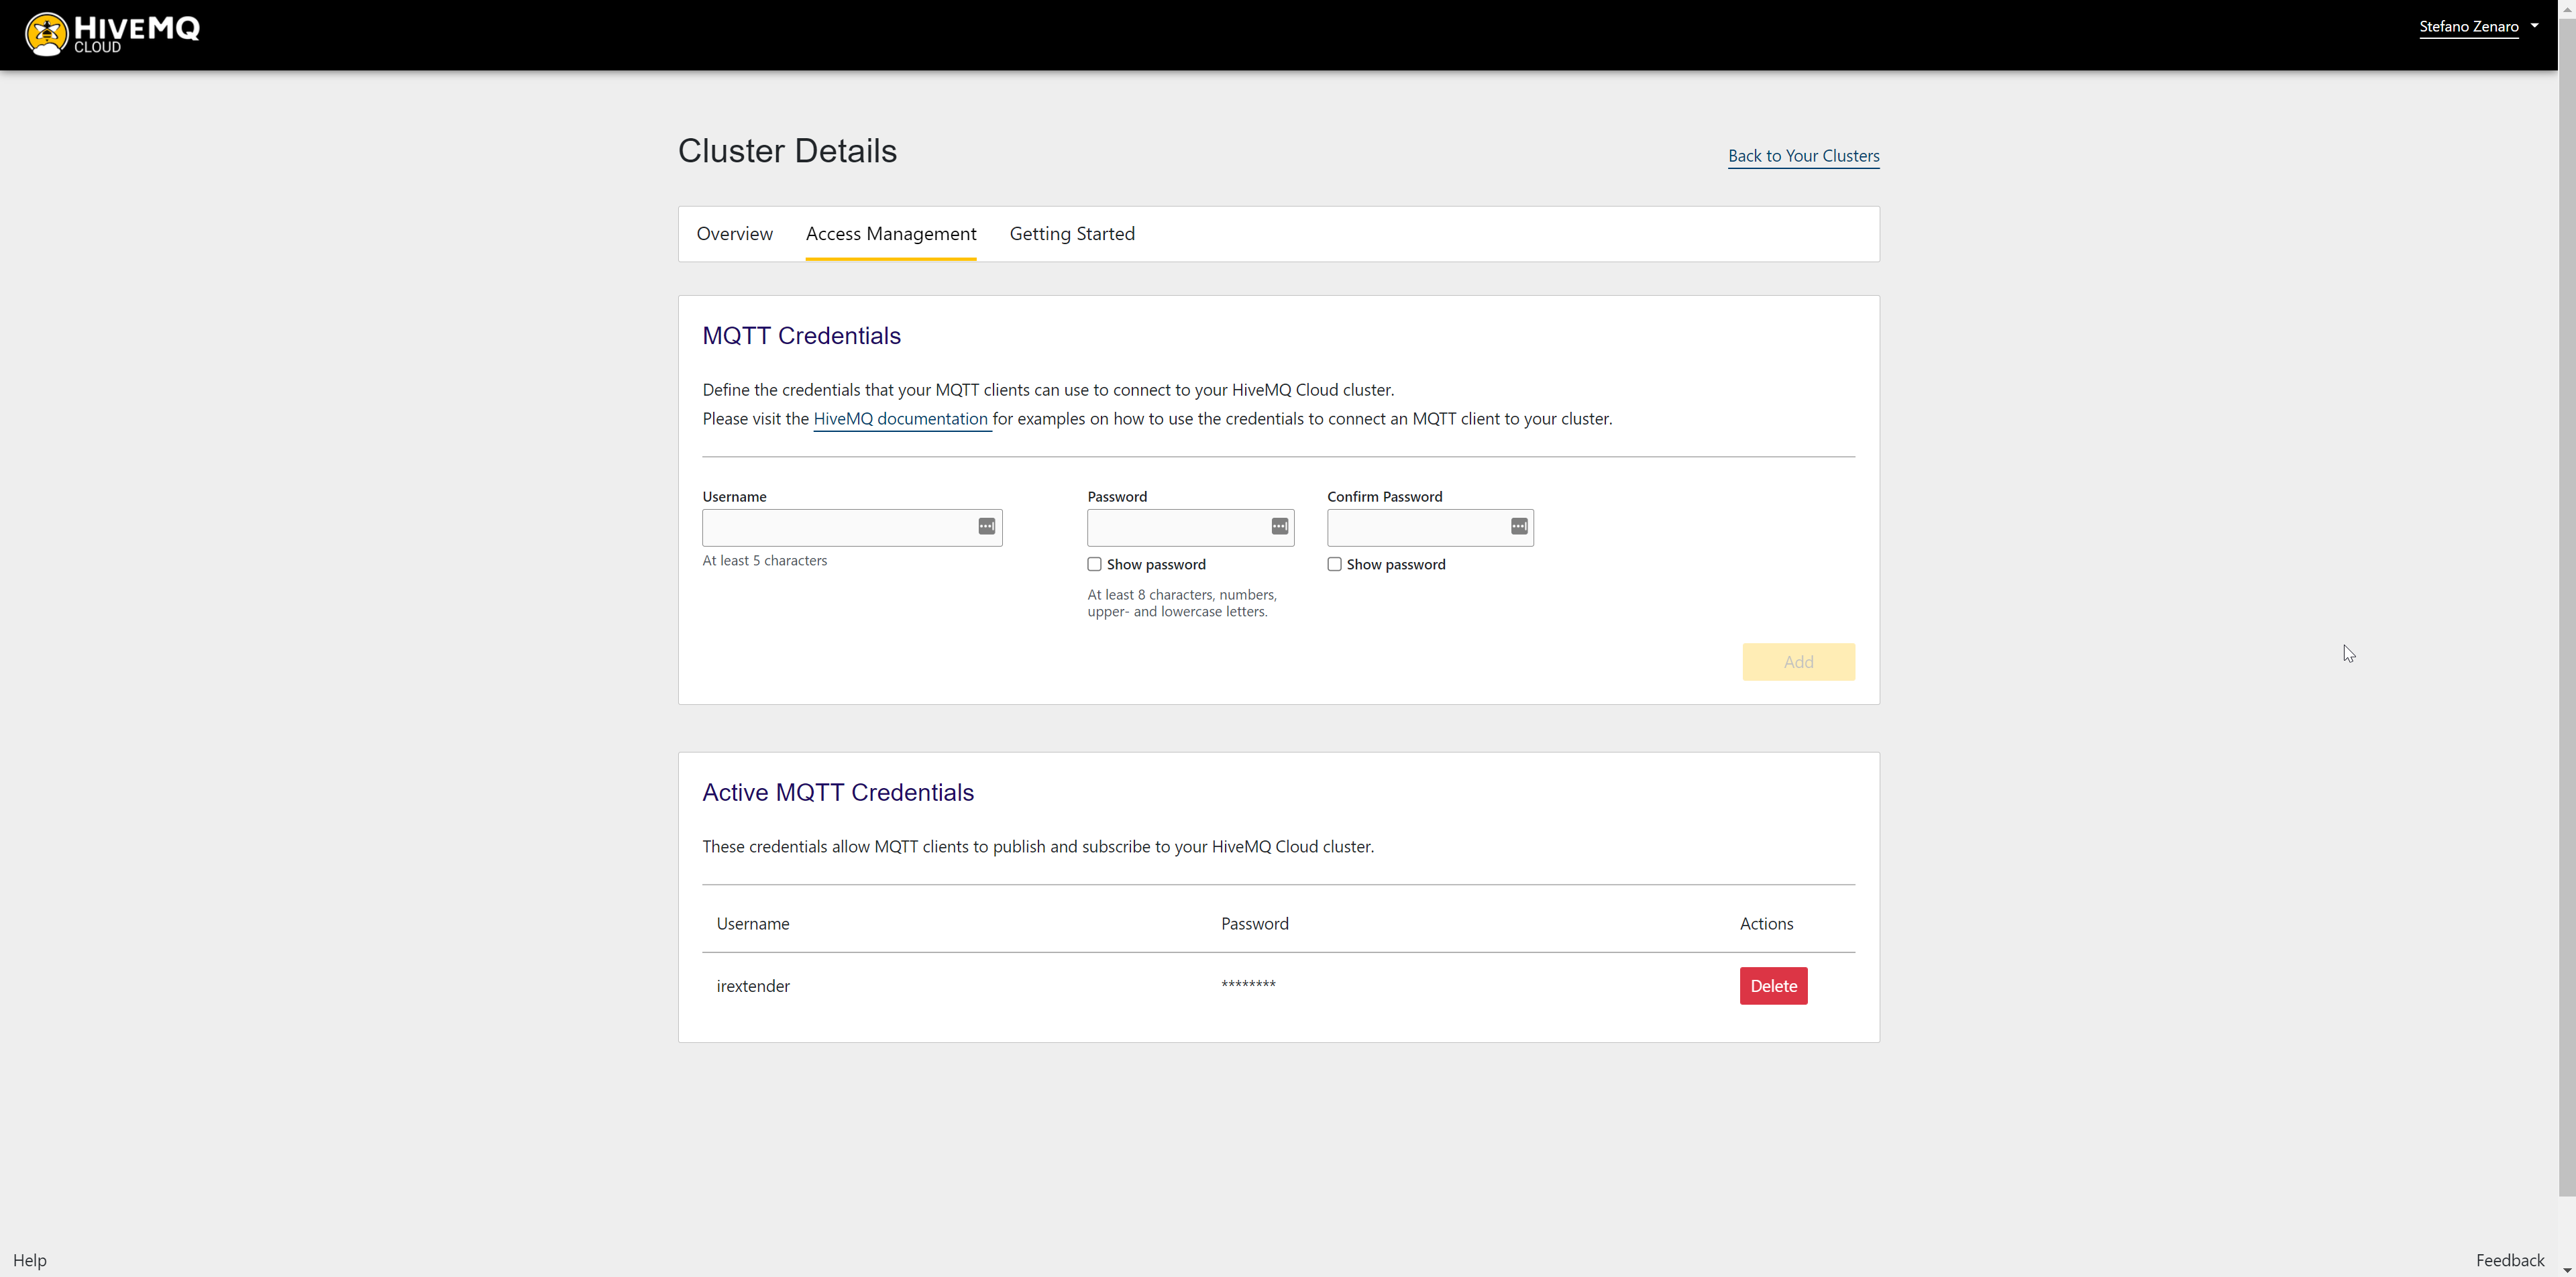
\includegraphics[width=0.8\textwidth,height=\textheight,keepaspectratio]{assets/hivemq_access_management}
        \end{figure}

    \end{enumerate}
\clearpage

% List of figures
\listoffigures
\addcontentsline{toc}{section}{\listfigurename}

\end{document}
